%%%%%%%%%%%%%%%%%%%%%%%%%%%%%%%%%%%%%%%%%%%%%%%%%%%%%%%%%%%%%%%%%%%%%%
%%  Copyright by Wenliang Du.                                       %%
%%  This work is licensed under the Creative Commons                %%
%%  Attribution-NonCommercial-ShareAlike 4.0 International License. %%
%%  To view a copy of this license, visit                           %%
%%  http://creativecommons.org/licenses/by-nc-sa/4.0/.              %%
%%%%%%%%%%%%%%%%%%%%%%%%%%%%%%%%%%%%%%%%%%%%%%%%%%%%%%%%%%%%%%%%%%%%%%

\newcommand{\commonfolder}{../../common-files}
\documentclass[11pt]{article}

\usepackage[most]{tcolorbox}
\usepackage{times}
\usepackage{epsf}
\usepackage{epsfig}
\usepackage{amsmath, alltt, amssymb, xspace}
\usepackage{wrapfig}
\usepackage{fancyhdr}
\usepackage{url}
\usepackage{verbatim}
\usepackage{fancyvrb}
\usepackage{adjustbox}
\usepackage{listings}
\usepackage{color}
\usepackage{subfigure}
\usepackage{cite}
\usepackage{sidecap}
\usepackage{pifont}
\usepackage{mdframed}
\usepackage{textcomp}
\usepackage{enumitem}


% Horizontal alignment
\topmargin      -0.50in  % distance to headers
\oddsidemargin  0.0in
\evensidemargin 0.0in
\textwidth      6.5in
\textheight     8.9in 

\newcommand{\todo}[1]{
\vspace{0.1in}
\fbox{\parbox{6in}{TODO: #1}}
\vspace{0.1in}
}


\newcommand{\unix}{{\tt Unix}\xspace}
\newcommand{\linux}{{\tt Linux}\xspace}
\newcommand{\minix}{{\tt Minix}\xspace}
\newcommand{\ubuntu}{{\tt Ubuntu}\xspace}
\newcommand{\setuid}{{\tt Set-UID}\xspace}
\newcommand{\openssl} {\texttt{openssl}}


\pagestyle{fancy}
\lhead{\bfseries SEED Labs}
\chead{}
\rhead{\small \thepage}
\lfoot{}
\cfoot{}
\rfoot{}


\definecolor{dkgreen}{rgb}{0,0.6,0}
\definecolor{gray}{rgb}{0.5,0.5,0.5}
\definecolor{mauve}{rgb}{0.58,0,0.82}
\definecolor{lightgray}{gray}{0.90}


\lstset{%
  frame=none,
  language=,
  backgroundcolor=\color{lightgray},
  aboveskip=3mm,
  belowskip=3mm,
  showstringspaces=false,
%  columns=flexible,
  basicstyle={\small\ttfamily},
  numbers=none,
  numberstyle=\tiny\color{gray},
  keywordstyle=\color{blue},
  commentstyle=\color{dkgreen},
  stringstyle=\color{mauve},
  breaklines=true,
  breakatwhitespace=true,
  tabsize=3,
  columns=fullflexible,
  keepspaces=true,
  escapeinside={(*@}{@*)}
}

\newcommand{\newnote}[1]{
\vspace{0.1in}
\noindent
\fbox{\parbox{1.0\textwidth}{\textbf{Note:} #1}}
%\vspace{0.1in}
}


%% Submission
\newcommand{\seedsubmission}{You need to submit a detailed lab report, with screenshots,
to describe what you have done and what you have observed.
You also need to provide explanation
to the observations that are interesting or surprising.
Please also list the important code snippets followed by
explanation. Simply attaching code without any explanation will not
receive credits.}

%% Book
\newcommand{\seedbook}{\textit{Computer \& Internet Security: A Hands-on Approach}, 2nd
Edition, by Wenliang Du. See details at \url{https://www.handsonsecurity.net}.}

%% Videos
\newcommand{\seedisvideo}{\textit{Internet Security: A Hands-on Approach},
by Wenliang Du. See details at \url{https://www.handsonsecurity.net/video.html}.}

\newcommand{\seedcsvideo}{\textit{Computer Security: A Hands-on Approach},
by Wenliang Du. See details at \url{https://www.handsonsecurity.net/video.html}.}

%% Lab Environment
\newcommand{\seedenvironment}{This lab has been tested on our pre-built
Ubuntu 16.04 VM, which can be downloaded from the SEED website. }

\newcommand{\seedenvironmentA}{This lab has been tested on our pre-built
Ubuntu 16.04 VM, which can be downloaded from the SEED website. }

\newcommand{\seedenvironmentB}{This lab has been tested on our pre-built
Ubuntu 20.04 VM, which can be downloaded from the SEED website. }

\newcommand{\seedenvironmentAB}{This lab has been tested on our pre-built
Ubuntu 16.04 and 20.04 VMs, which can be downloaded from the SEED website. }

\newcommand{\nodependency}{Since we use containers to set up the lab environment, 
this lab does not depend too much on our SEED VM. You can do this lab
using other VMs or physical machines. }







\newcommand{\seedlabcopyright}[1]{
\vspace{0.1in}
\fbox{\parbox{6in}{\small Copyright \copyright\ {#1}\ \ by Wenliang Du.\\
      This work is licensed under a Creative Commons
      Attribution-NonCommercial-ShareAlike 4.0 International License.
      If you remix, transform, or build upon the material, 
      this copyright notice must be left intact, or reproduced in a way that is reasonable to
      the medium in which the work is being re-published.}}
\vspace{0.1in}
}





% Many labs reference the section numbers of the manual. If those numbers
% are changed, we need to change this file, otherwise, the reference will
% be out of sync.

\newcommand{\manualonelan}{1}
\newcommand{\manualtwolan}{2}
\newcommand{\manualdns}{3}
\newcommand{\manualnaming}{4}
\newcommand{\manualproblem}{5}



\lhead{\bfseries SEED Labs -- IP/ICMP Attacks Lab}
\newcommand{\ipFigs}{./Figs}


\begin{document}



\begin{center}
{\LARGE IP/ICMP Attacks Lab}
\end{center}

\seedlabcopyright{2020}


% *******************************************
% SECTION
% ******************************************* 
\section{Overview}

The objective of this lab is for students to gain the first-hand experience 
on various attacks at the IP layer. Some of the attacks may not work anymore,
but their underlying techniques are quite generic, and it
is important for students to learn these attacking techniques, so when they design
or analyze network protocols, they are aware of what attackers can do to protocols.
Moreover, due to the complexity of IP fragmentation, spoofing fragmented IP packets
is non-trivial.  Constructing spoofed 
IP fragments is a good practice for students to hone their
packet spoofing skills, which are essential in network security.  
We will use Scapy to conduct packet spoofing.  
This lab covers the following topics:

\begin{itemize}[noitemsep]
\item The IP and ICMP protocols
\item IP Fragmentation and the related attacks
\item ICMP redirect attack
\item Routing 
\end{itemize}



\paragraph{Videos.}
Detailed coverage of the IP protocol and the attacks at the IP layer can be found 
in the following:

\begin{itemize}
\item Section 4 of the SEED Lecture, \seedisvideo
\end{itemize}


\paragraph{Lab environment.} \seedenvironmentB


% *******************************************
% SECTION
% ******************************************* 
\section{Tasks 1: IP Fragmentation}

Two VMs are needed for this task. They should be connected to the same network, so they
can communicate with each other.

% -------------------------------------------
% SUBSECTION
% ------------------------------------------- 
\subsection{Task 1.a: Conducting IP Fragmentation}

In this task, students need to construct a UDP packet and send it to a UDP 
server. They can use \texttt{"nc -lu 9090"} to start a UDP server. 
Instead of building one single IP packet, students need to 
divide the packet into 3 fragments, each containing 32 bytes of data (the
first fragment contains 8 bytes of the UDP header plus 32 bytes of data).
If everything is done correctly, the server will display
96 bytes of data in total.  
The following is a sample code for constructing the first fragment.

\begin{lstlisting}
#!/usr/bin/python3
from scapy.all import *

# Construct IP header
ip = IP(src="1.2.3.4", dst="10.0.0.15")
ip.id    = 1000  # Identification
ip.frag  = 0     # Offset of this IP fragment
ip.flags = 1     # Flags

# Construct UDP header
udp = UDP(sport=7070, dport=9090)
udp.len  = 200   # This should be the combined length of all fragments

# Construct payload
payload = 'A' * 80    # Put 80 bytes in the first fragment

# Construct the entire packet and send it out
pkt = ip/udp/payload  # For other fragments, we should use ip/payload
pkt[UDP].checksum = 0 # Set the checksum field to zero
send(pkt, verbose=0)
\end{lstlisting}


It should be noted that the UDP checksum field needs to be set 
correctly. If we do not set this field, Scapy will calculate 
the checksum for us, but this checksum will only be based on the 
data in the first fragment, which is incorrect.
If we set the checksum field to  zero, Scapy will leave it alone.
Moreover, the recipient will not validate the UDP checksum 
if it sees a zero in the checksum field, 
because in UDP, checksum validation is optional.


If you use Wireshark to observe traffic, it should also be noted that by default, 
Wireshark will reassemble fragments in the last fragment packet and
show it as a complete IP/UDP packet. To change that behavior,
we should disable IP fragment reassembly in Wireshark preferences.
Click the following menu sequence: \texttt{Edit} $\rightarrow$ \texttt{Preferences}; 
click the \texttt{Protocols} dropdown menu, find and click \texttt{IPv4}.
Uncheck the \texttt{"Reassemble fragmented IPv4 datagrams"} option. 




% -------------------------------------------
% SUBSECTION
% ------------------------------------------- 
\subsection{Task 1.b: IP Fragments with Overlapping Contents}

Similar to Task 1.a, students also need to construct 3 fragments to send data to a UDP server.
The size of each fragment is up to students.  The objective of this task is to create
overlapping fragments.  In particular, the first two fragments should overlap.  Please use
experiments to show what will happen when the overlapping occurs. Please
try the following overlapping scenarios separately:
 
 \begin{itemize} 
 \item The end of the first fragment and the beginning of the second
 fragment should have \texttt{K} bytes of overlapping, i.e., the last  
 \texttt{K} bytes of data in the first fragment should have the same
 offsets as the first \texttt{K} bytes of data in the second fragment. 
 The value of \texttt{K} is decided by students (\texttt{K} should be 
 greater than zero and smaller than the size of either fragment). In the reports, students
 should indicate what their \texttt{K} values are. 


 \item The second fragment is completely enclosed in the first fragment.
 The size of the second fragment must be smaller than the 
 first fragment (they cannot be equal).

 \end{itemize} 


Please try two different orders: (1) sending the first fragment first, and 
(2) sending the second fragment first. Please report whether the results will
be the same. 





% -------------------------------------------
% SUBSECTION
% ------------------------------------------- 
\subsection{Task 1.c: Sending a Super-Large Packet}

As we know, the maximal size for an IP packet is $2^{16}$ octets, because
the length field in the IP header has only 16 bits. 
However,
using the IP fragmentation, we can create an IP packet that 
exceeds this limit. Please construct such a packet, send
it to the UDP server, and see how the server responds to this 
situation. Please report your observation. 
  



% -------------------------------------------
% SUBSECTION
% ------------------------------------------- 
\subsection{Task 1.d: Sending Incomplete IP Packet}


In this task, we are going to use Machine A to launch a Denial-of-Service attack 
on Machine B. In the attack, Machine A sends  a lot of 
incomplete IP packets to B, i.e., these packets consist of 
IP fragments, but some fragments are missing. All these incomplete IP packets 
will stay in the kernel, until they time out. Potentially, this can
cause the kernel to commit a lot of kernel memory. In the past, this 
had resulted in denial-of-service attacks on the server. Please try 
this attack and describe your observation. 




% *******************************************
% SECTION
% ******************************************* 
\section{Task 2: ICMP Redirect Attack}

An ICMP redirect is an error message sent by a router to the sender of an
IP packet. Redirects are used when a router believes a packet is being
routed incorrectly, and it would like to inform the sender that it should
use a different router for the subsequent packets sent to that same
destination.


In our VM, there is a countermeasure against the ICMP redirect attack. Before doing
the task, we need to turn off the countermeasure by configuring the operating system
to accept ICMP redirect messages. 

\begin{lstlisting}
$ sudo sysctl net.ipv4.conf.all.accept_redirects=1
\end{lstlisting}

For this task, we should have two VMs, the victim VM (Host A) and 
the attacker VM (Host M). Students should pick a destination B, which
should be a host outside of our local network (e.g., an outside web server). 
Normally, when A sends a packet to B, the packet will go to the 
router provided by VirtualBox (usually it is \texttt{10.0.2.1} if we use
the default IP prefix for NAT Network). 

The objective of this task is to launch an ICMP redirect attack on Host A 
from Host M, such that when Host A sends packets to B, 
it will use M as the router, and hence sends those packets to M. 
Since M is controlled by the attacker, the attacker can 
intercept the packets, make changes, and then send 
the modified packets out. This is a form of the Man-In-The-Middle (MITM) attack. 
For the simplicity of this lab, students are not required to 
conduct the MITM part; they only need to demonstrate that 
their ICMP redirect attacks can successfully redirect
packets from A to B.


\paragraph{Code skeleton.} A code skeleton is provided in the following, with
some of the essential parameters left out. Students should fill in the proper 
values in the places marked by \texttt{@@@@}.  


\begin{lstlisting}
#!/usr/bin/python3

from scapy.all import *

ip = IP(src = @@@@,  dst = @@@@)
icmp = ICMP(type=@@@@, code=@@@@)
icmp.gw = @@@@

# The enclosed IP packet should be the one that 
# triggers the redirect message. 
ip2 = IP(src = @@@@, dst = @@@@)
send(ip/icmp/ip2/UDP());
\end{lstlisting}
 

\paragraph{Verification.}
To verify whether the ICMP redirect attack is successful, we can use 
the \texttt{"ip route get"} command to see what router will be used for a 
packet destination. For example, if we want to know
what router will be used for packets going to \texttt{8.8.8.8}, we can use 
the following command: 

\begin{lstlisting}
$ ip route get 8.8.8.8
8.8.8.8 via 10.0.2.1 dev enp0s3  src 10.0.2.4
    cache
\end{lstlisting}


\paragraph{Questions.} Please conduct the following experiments, and explain your observations:

\begin{enumerate}
\item Can you use ICMP redirect attacks to redirect to a remote machine? Namely,
the IP address assigned to \texttt{icmp.gw} is a computer not on the local LAN. 
Please show your experiment result, and explain your observation.  

\item Can you use ICMP redirect attacks to redirect to a non-existing machine on
the same network? Namely, the IP address assigned to \texttt{icmp.gw} is a local computer that
is either offline or non-existing. 
Please show your experiment result, and explain your observation.  
\end{enumerate}





% *******************************************
% SECTION
% ******************************************* 
\section{Task 3: Routing} 


The objective of this task is for students to get familiar with routing. 
Even though this task is not relevant to security, it is essential
for many network-related SEED labs, so we will cover it
in this lab. 
We need at least three machines 
and two networks for this lab (see Figure~\ref{fig:setup}). 
There are two approaches to set up this lab environment. 
One is to use VirtualBox to create virtual machines and networks. 
Another approach is to use Docker to create containers and networks. 
We do encourage students to use 
the Docker approach, because it is much more convenient to set up.


\begin{figure}[htb]
\begin{center}
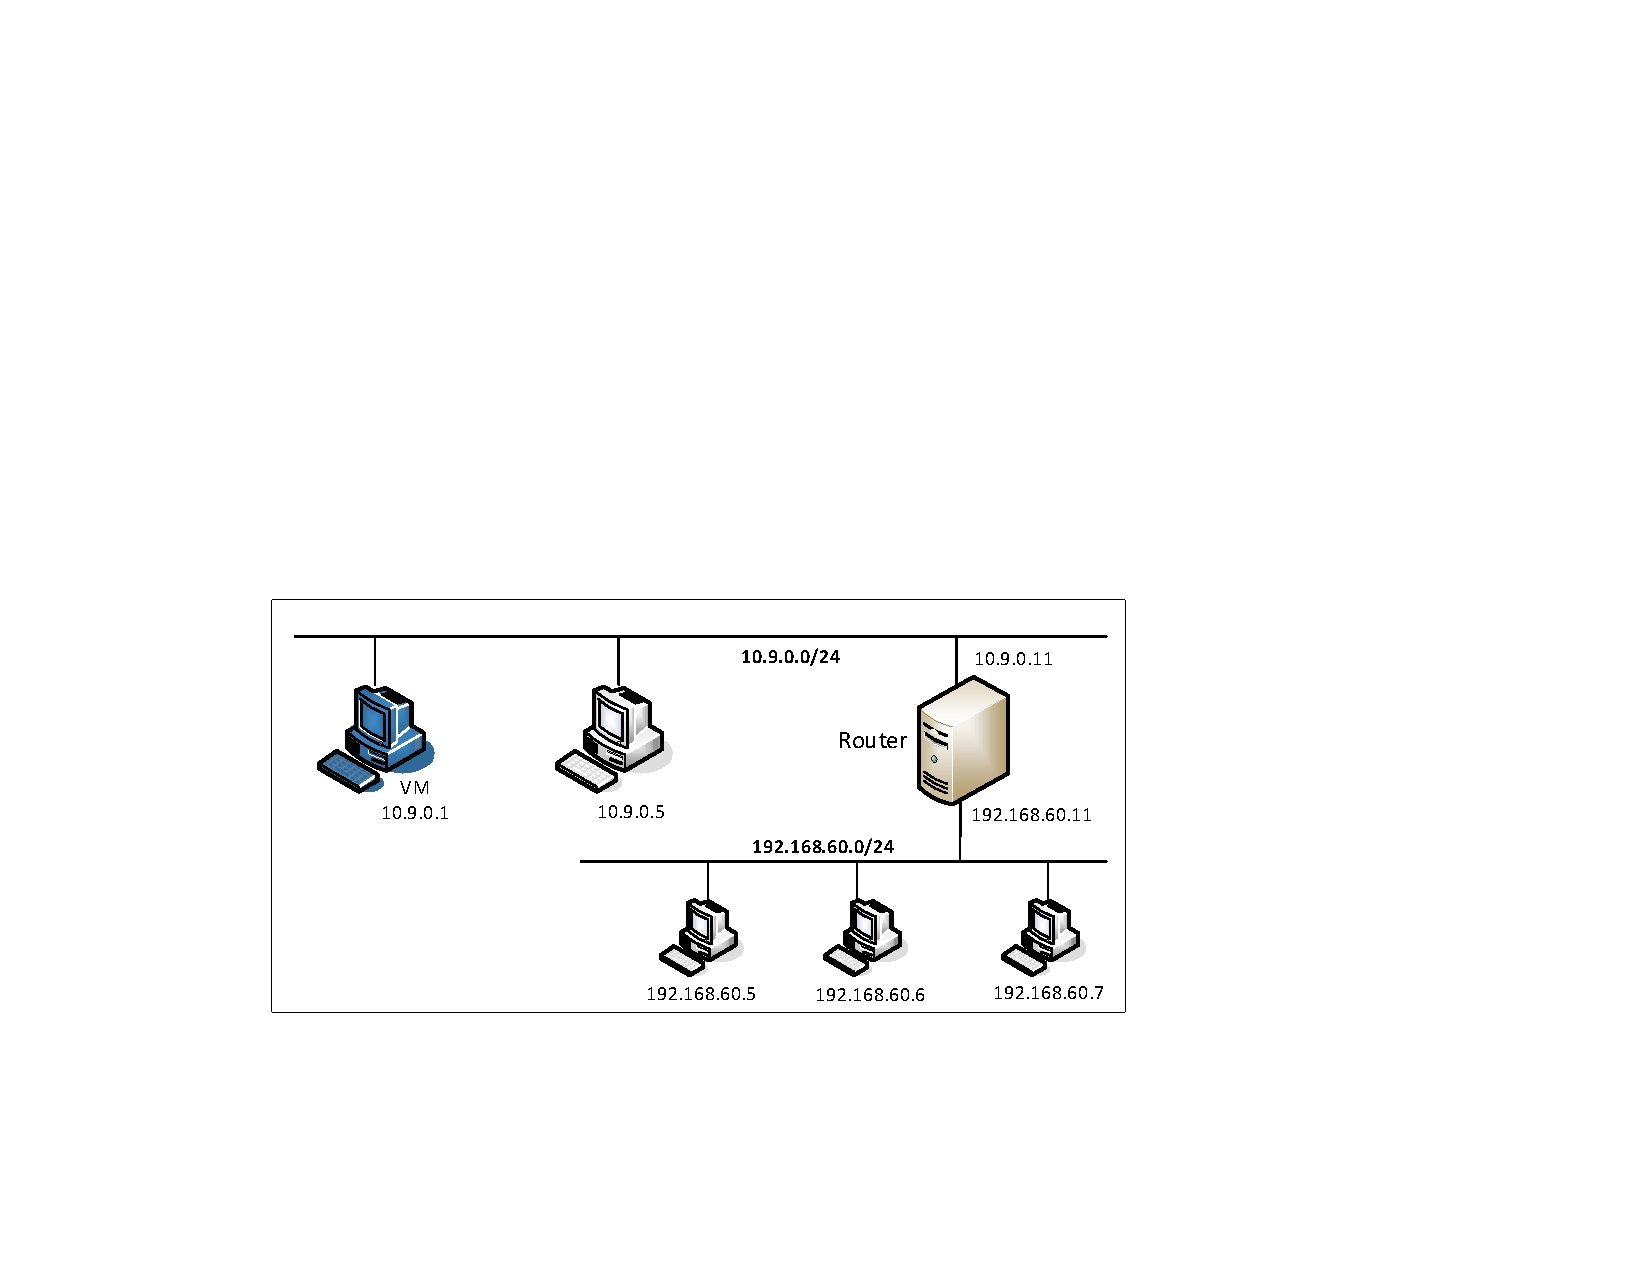
\includegraphics[width=0.8\textwidth]{\commonfolder/Figs/TwoLANs.pdf}
\end{center}
\caption{Lab environment setup}
\label{fig:setup}
\end{figure}


%%%%%%%%%%%%%%%%%%%%%%%%%%%%%%%%%%%%%%%%%%%%
% Input common files related to containers

\paragraph{Container setup and commands.}



The Docker and Compose files, along with the user manual,
can be downloaded from the lab's website,
The followings Compose commands are for creating and tearing down
the lab environment. 
Since we are going to use 
these commands and several docker commands very
frequently, we have created aliases for these commands
in the \texttt{.bashrc} file.  


\begin{lstlisting}
$ docker-compose build  # Build the container image
$ docker-compose up     # Start the container
$ docker-compose down   # Shut down the container

// Aliases for commonly used docker and Compose commands. 
$ dcbuild       # Alias for: docker-compose build
$ dcup          # Alias for: docker-compose up
$ dcdown        # Alias for: docker-compose down
$ dockps        # Alias for: docker ps --format "{{.ID}}  {{.Names}}" 
$ docksh <id>   # Alias for: docker exec -it <id> /bin/bash
\end{lstlisting}



Detailed explanation of \texttt{Dockerfile} and
the \texttt{docker-compose.yml} file can be found from
the manual, which is linked to this lab's website. If you encounter
issues when setting up the lab environment, read the
``Common Problems'' section for potential solutions.



\paragraph{Removing the Host VM from \texttt{192.168.60.0/24} network.}
When Docker creates a network, it automatically attach the
host machine (i.e., the VM) to the network. In this
case, the host machine is attached to both
networks, and is given the IP address \texttt{10.9.0.1} and
\texttt{192.168.60.1}.
This may create undesirable situations,
so let's remove it.

In our setup, we only want the VM to be connected to
\texttt{10.9.0.0/24}, not to both.
We need to detach the VM from the other network. We cannot simply power down
the interface, because that will affects all the containers on that network.
Our solution is to remove the IP address
of the interface, and then set the routing accordingly. The following
script does exactly that.


\begin{lstlisting}
#!/bin/bash

# Get the interface name
IFname=$(docker network ls | grep 192.168.60.0 | cut -d' ' -f 1)

# Remove the IP address from the interface
sudo ip addr flush br-$IFname

# Use 10.9.0.11 as the router to access 192.168.60.0/24
sudo ip route add 192.168.60.0/24 via 10.9.0.11
\end{lstlisting}


%%%%%%%%%%%%%%%%%%%%%%%%%%%%%%%%%%%%%%%%%%%%


\paragraph{Note on Router configuration.}
Unless specifically configured, a computer will only act as a host,
not as a gateway, i.e., they do not forward packets for 
others. For the router container to function like a router,
we need to enable the IP forwarding on it. 
For virtual machines, we can use the following 
command to enable IP forwarding on the VM:

\begin{lstlisting}
$ sudo sysctl net.ipv4.ip_forward=1
\end{lstlisting}

However, for containers, we are not able to run this command. 
Even though we have a root account, this root is not the 
same as that on the hosting VM, and there 
are certain things that we cannot do inside the container, such as 
modifying this variable and alike. If we run the command,
we will see the following error message. The container
is not given the privilege to make the change.

\begin{lstlisting}
# sysctl net.ipv4.ip_forward=1
sysctl: setting key "net.ipv4.ip_forward": Read-only file system
\end{lstlisting}

If we want to modify this flag for a container,
we have to do it when we build the container.
That is why we added the following entry
to the \texttt{docker-compose.yml} file:

\begin{lstlisting}
sysctls:
         - sysctl net.ipv4.ip_forward=1
\end{lstlisting}



\paragraph{Task.} After we have set up the containers and 
networks, hosts on the same LAN can communicate with one another, but
not the hosts on different LANs. This is because we have not set 
up the routing on the router and hosts yet. This task is left 
to students. Students need to configure the routing table 
on all the containers, so the can communicate with one 
another. 

There are two approaches to configure the routing table
on containers. One is to get on each running container, and manually configure its routing
table. Another approach is to add commands to the Compose file (\texttt{docker-compose.yml}), 
so when each container is started, the commands will be automatically
executed. We do recommend students to use the Compose file approach. 
Students can find the \texttt{command} entry for some of the 
containers. Since a command entry only allows one command,
if we want to execute multiple commands, we feed the command
string (commands are separated by \texttt{\&\&}) 
to the \texttt{"bash -c"} command for execution.

\begin{lstlisting}
command: bash -c "
             command one && 
	     command two && 
	     command three
         "
\end{lstlisting}
 

Routing tables can be set using the \texttt{ip route} command. Students who are not familiar 
with this command can easily find its manual on the Internet. We list 
some of the usage examples in the following:

\begin{lstlisting}
// List all the entries in the routing table 
# ip route 

// Add an entry 
# ip route add <network> dev <interface> via <router ip>

// Delete a routing entry
# ip route del ...
\end{lstlisting}



% *******************************************
% SECTION
% ******************************************* 
\section{Submission}

\seedsubmission

\end{document}



